\section{Transdutores e Atuadores}

Os transdutores a atuadores foram escolhidos primeiramente visando atingir os objetivos propostos, mas também visando uma diversidade de circuitos de condicionamento de sinal necessários. Dessa forma, aproveitou-se do caráter virtual do projeto para que fossem experimentados diferentes abordagens.

Para o projeto dos circuitos de condicionamento, imaginou-se uma placa de aquisição e acionamento com limites de operação entre 0\,V e 5\,V, alta impedância e baixa potência de saída.

\subsection{Transdutores}

\subsubsection{Transdutores de temperatura}

\paragraph{Escolha dos componentes}\mbox{}

Para os transdutores de temperatura TI 01 a 05 foram escolhidos PT100, uma vez que possuem ampla utilização e possuem resposta suficiente para a aplicação, ou seja, sua sensibilidade na faixa de temperatura desejada é suficiente e não possui tempo de resposta impeditivo para um controle de temperatura.

De forma mais específica, o TRA-C61, da OPTITEMP foi selecionado uma vez que é um PT100 de Classe A e possui um tempo de resposta $t_{95\%} = 8,0$\,s. Além disso, possui já encapsulamento adequado para contato com alimentos. Ressalta-se que o ambiente do projeto é adequado também ao elemento sensor, uma vez que ele não sofrerá impactos no interior do tanque e também não haverá grande agitação.

\paragraph{Circuito de condicionamento}\mbox{}

Para condicionamento do sinal dos transdutores selecionados, utilizou-se uma medição a 4 fios e uma fonte de corrente. A queda de tensão sobre o PT100, então, alimenta um primeiro estágio de amplificação de diferenças para eliminar o \emph{offset} causado pela resistência de fio e um segundo estágio para eliminar o \emph{offset} padrão do PT100 e mapear a variação de 0\,ºC a 100\,ºC na faixa de 0\,V a 5\,V. Os resultados podem ser vistos na figura abaixo.

\begin{figure}[H]
    \centering
    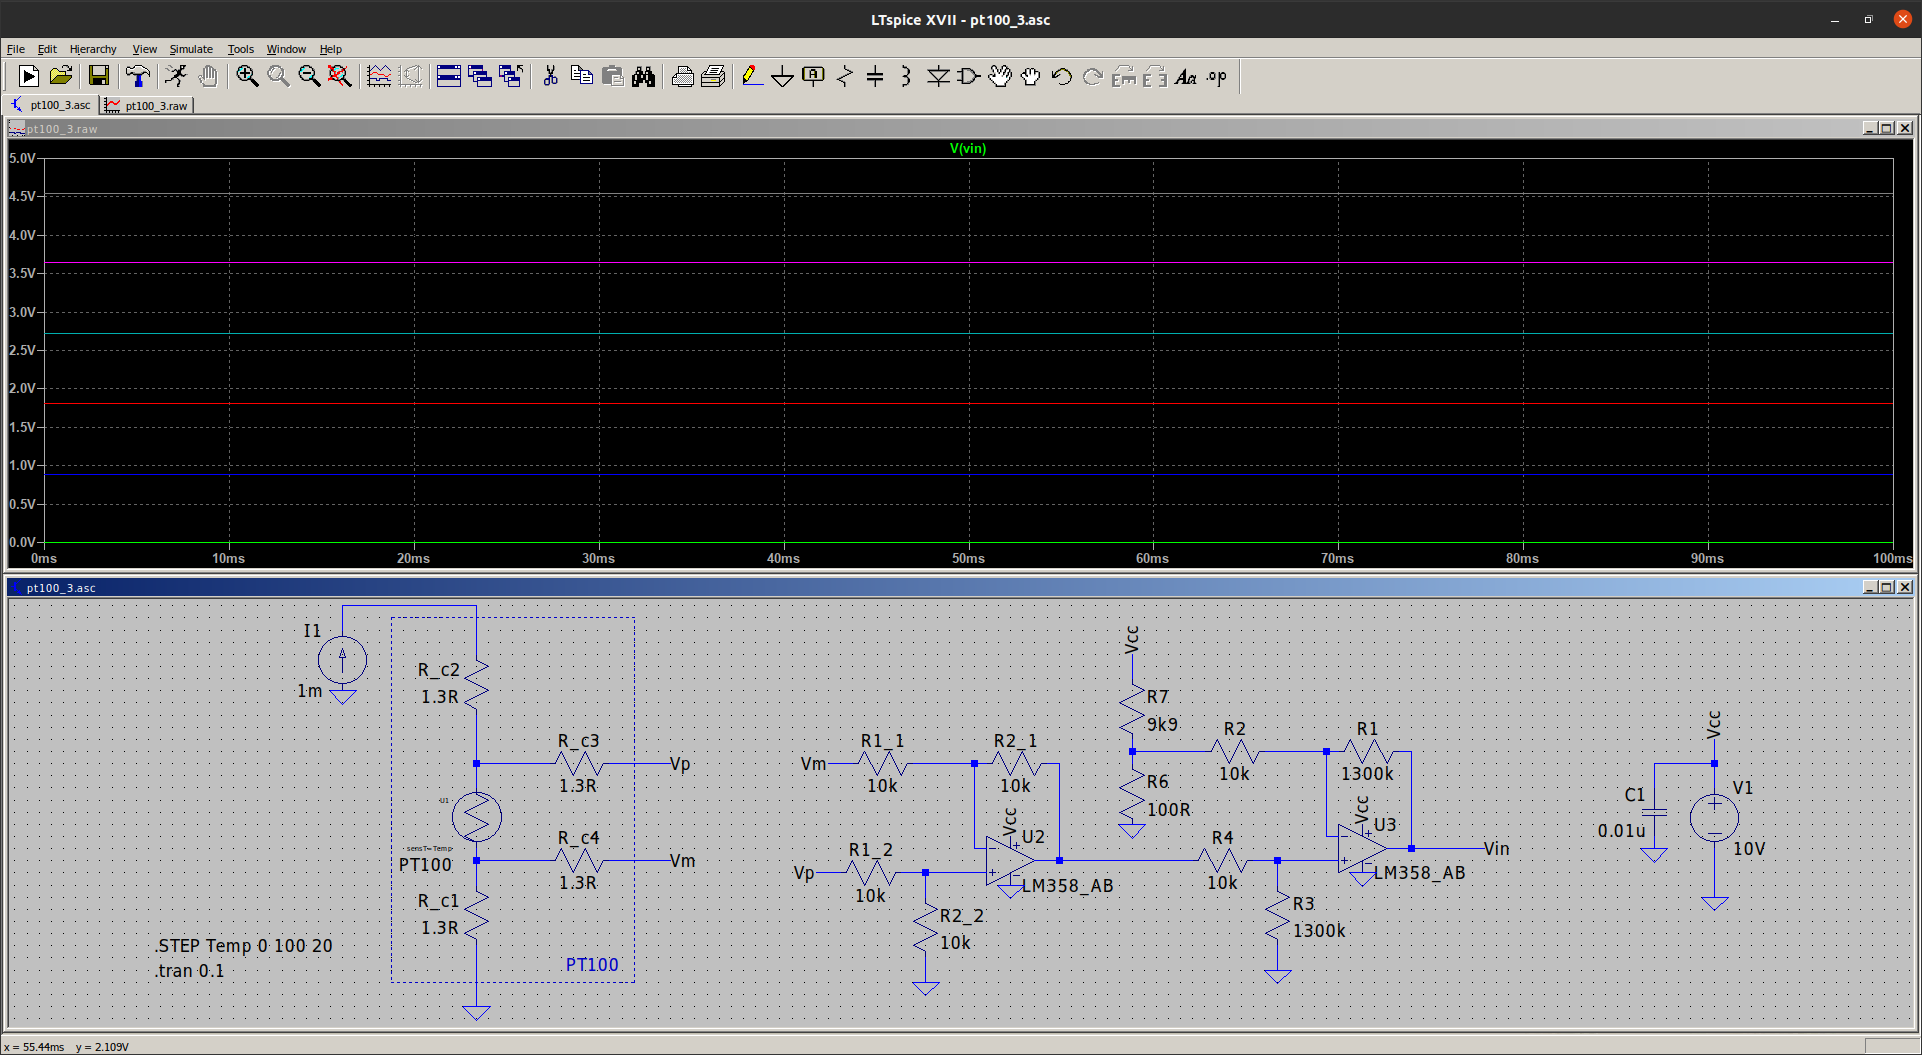
\includegraphics[width=0.8\textwidth]{imagens/temp_circ.png}
    \caption{Circuito de condicionamento de sinal do transdutor de temperatura e resultados da simulação. O nó \emph{Vin} simula a porta de leitura analógica do sistema de aquisição.}
    \label{fig:imagens-temp_circ-png}
\end{figure}

Como pode ser visto, os resultados ficaram cerca de 10\% abaixo do esperado. Essa variação também foi observada diretamente em cima do componente do transdutor, portanto, imagina-se que sejam causadas por parâmetros do próprio modelo SPICE do componente.

\paragraph{Simulação}\mbox{}

Para integrar o transdutor à simulação da planta, de forma a simular a implementação real da instrumentação, o transdutor foi simulado como um sistema de primeira ordem discreto seguido pelo tratamento do sinal, convertendo a grandeza física medida em um sinal na faixa de tensão que seria lida.

\subsubsection{Transdutores de Nível}

\paragraph{Escolha dos componentes}\mbox{}

As grandes limitações para a escolha de um transdutor de nível são a grande faixa de medição e a adequação a líquidos. Transdutores que se encaixam nessas restrições são transdutores potenciométricos de nível. Esses transdutores, muito utilizados em processos similares ao do escopo deste trabalho, comparam o potencial elétrico em uma haste metálica com a aquele da parede de um tanque ou de uma outra haste de referência. Dessa forma, eles fornecem rápida resposta, grande faixa de medição e suportam condições adversas.

O componente escolhido foi da série LSP-050.200.X.XXX, que possui uma haste de 2 metros e suporta variações de temperatura além daquelas do processo em questão. O transdutor tem tempo de resposta $t_{66\%} = 0,01$\,s, o que é muito além do necessário para a aplicação. Além disso, esse componente possui saída em corrente, em uma faixa de 4\,mA a 20\,mA, o que requer uma abordagem diferente para o condicionamento do sinal.

\paragraph{Circuito de condicionamento}\mbox{}

Para garantir a leitura adequada do sinal, um simples resistor foi utilizado para converter o sinal de corrente para tensão de forma que o sistema de aquisição pudesse realizar a leitura. A faixa de corrente do transdutor foi mapeada no intervalo de 1\,V a 5\,V. o \emph{offset} não foi compensado uma vez que o fabricante especifica que valores de corrente inferiores a 4\,mA indicam que o tanque está vazio, portanto, mapeadas em leituras a baixo de 1\,V. Além disso, não é um requisito a máxima resolução para o nível, não havendo perdas significativas para os resultados obtidos. O circuito projetado pode ser observado na figura abaixo, junto dos resultados da simulação.

\begin{figure}[H]
    \centering
    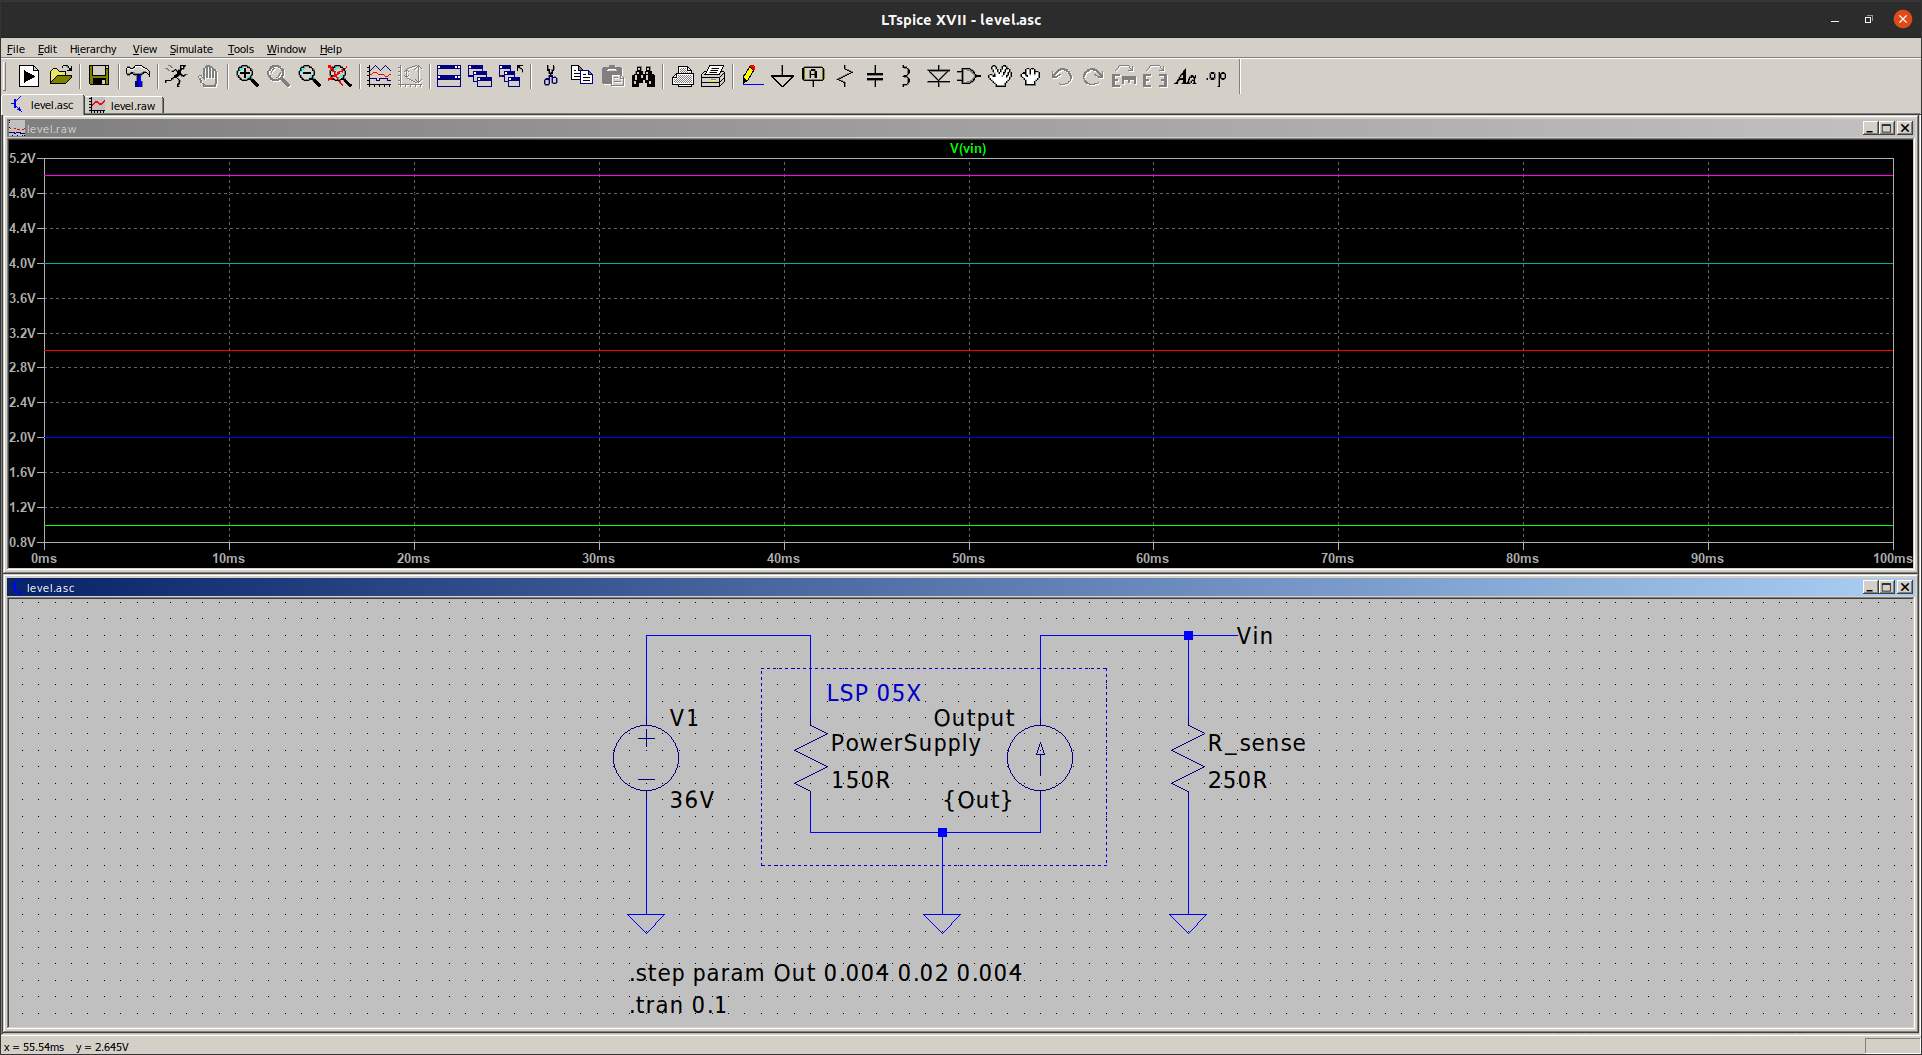
\includegraphics[width=0.8\textwidth]{imagens/level_circ.png}
    \caption{Circuito de condicionamento de sinal do transdutor de nível e resultados da simulação. O nó \emph{Vin} simula a porta de leitura analógica do sistema de aquisição.}
    \label{fig:imagens-level_circ-png}
\end{figure}

\paragraph{Simulação}\mbox{}

Ainda que bastante rápido frente os demais componentes do sistema, o transdutor de nível também foi simulado no LabVIEW como um sistema de primeira ordem seguido da conversão do nível de líquido para o sinal de tensão simulando o circuito de condicionamento.

\subsection{Atuadores}

\subsubsection{Aquecedor elétrico}

\paragraph{Escolha dos componentes}\mbox{}

A escolha de uma aquecedor elétrico adequado à aplicação passou pela necessidade do aquecimento de um grande volume de líquido, requerendo grande potência, e a simplicidade tanto do acionamento quando do modelo. Aquecedores de base, apesar de cogitados no início, não foram encontrados para tanques de grande porte. Soluções de aquecimento através de chamas também foram desconsideradas pela complexidade do acionamento e controle e por serem soluções sob medida, dificultando a obtenção dos parâmetros para modelagem.

Ao final, aquecedores submersíveis se mostraram alternativas bastante interessantes. São soluções altamente eficazes, uma vez que não há perda de calor para o ambiente, o que permite uma grande injeção de calor no líquido. O aquecedor TMT04014 foi tido como base, ainda que o modelo utilizado não tenha seguido fielmente as especificações do fabricante.

\paragraph{Circuito de condicionamento}\mbox{}

Como o aquecedor não possui sinais de controle, seu acionamento foi feito através da conexão com a rede elétrica. Para isso, um opto-DIAC foi utilizado para isolar a placa de controle da rede e um TRIAC em cascata foi utilizado para suportar a corrente do aquecedor e a tensão da rede. Os resultados podem ser observados na figura abaixo.

\begin{figure}[H]
    \centering
    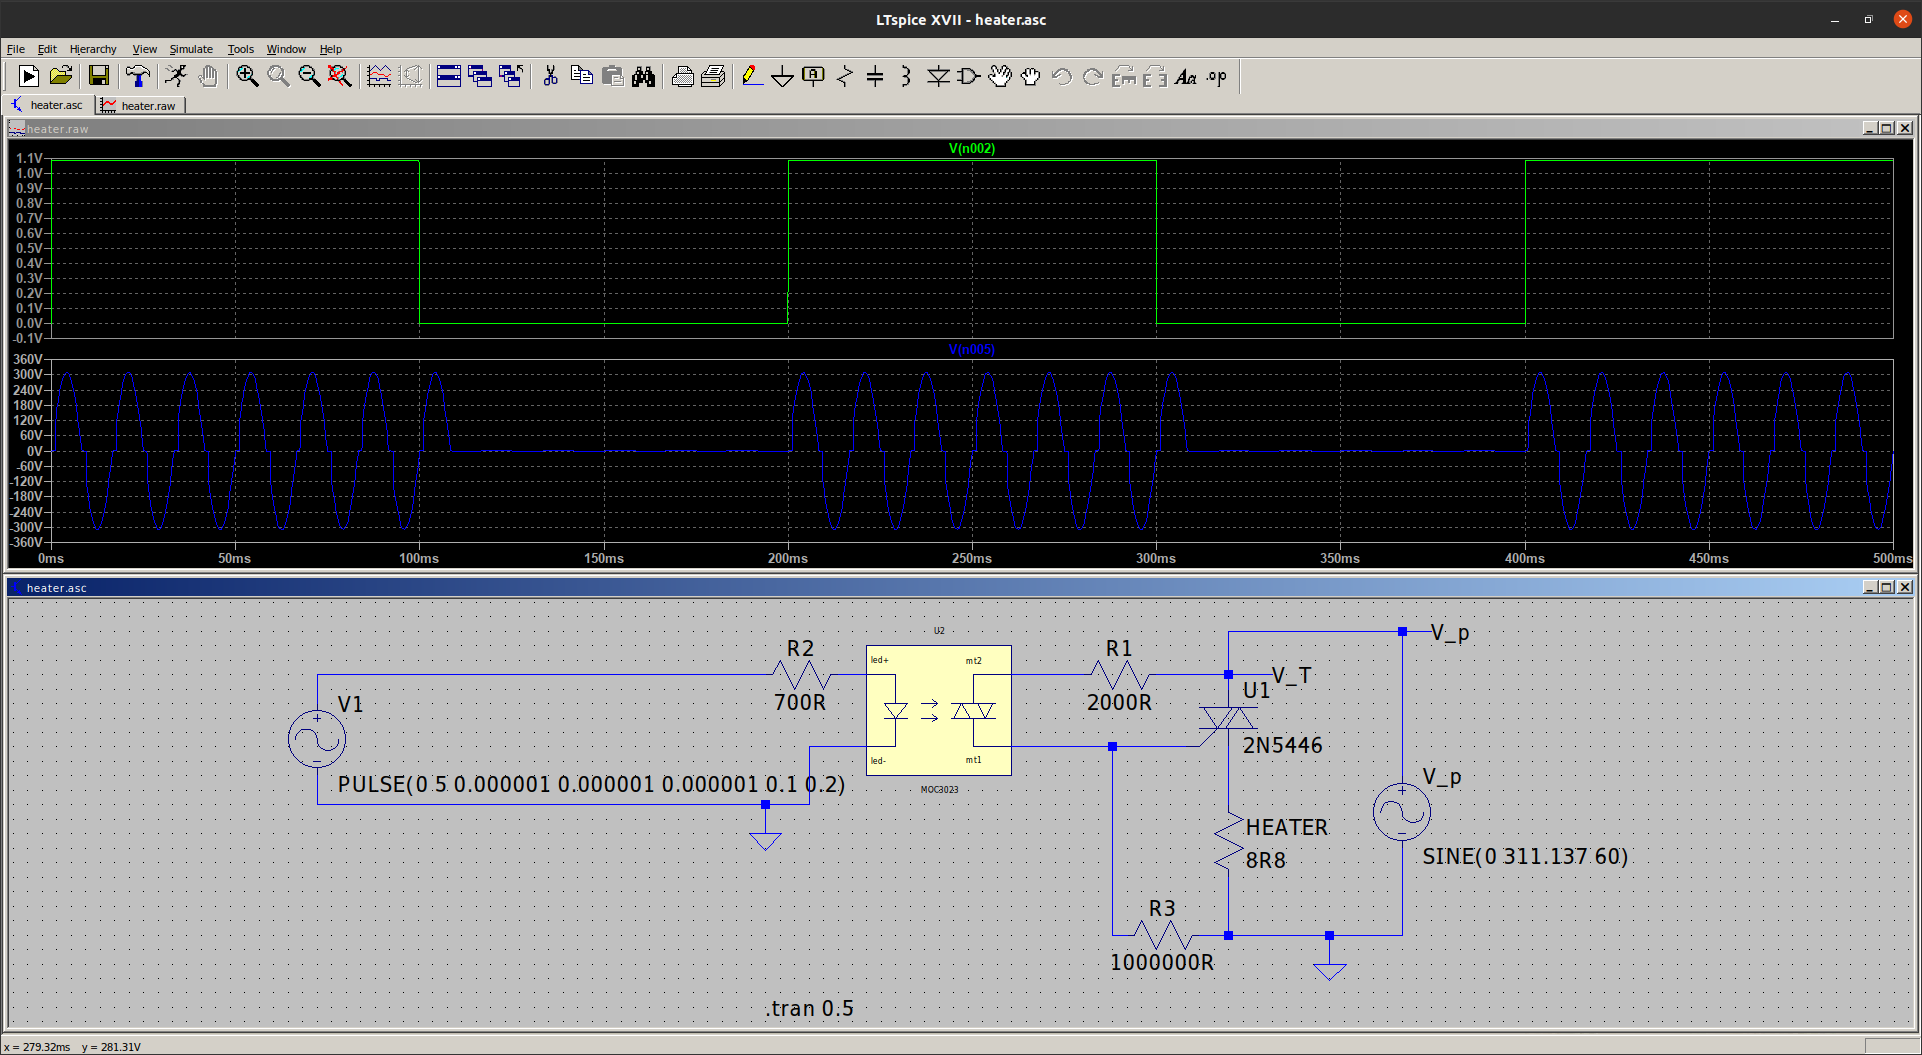
\includegraphics[width=0.8\textwidth]{imagens/heater_circ.png}
    \caption{Circuito de acionamento do aquecedor elétrico e resultados da simulação. A fonte \emph{V1} simula o sinal de saída da placa de controle, enquanto a fonte \emph{V\_p} simula a tensão da rede elétrica.}
    \label{fig:imagens-heater_circ-png}
\end{figure}

\paragraph{Simulação}\mbox{}

Infelizmente, a fabricante não disponibiliza o tempo de resposta do aquecedor. Dessa forma, assumiu-se que a potência consumida é imediatamente injetada no sistema, ou seja, desprezou-se o tempo de resposta. Ainda mais, a troca de calor utilizada no modelo do tanque como base para a simulação foi uma estimativa da gerada pelo aquecedor, uma vez que a modelagem de trocadores de calor foge do escopo deste trabalho. Dessa forma, o modelo no LabVIEW foi uma simples conversão do sinal binário do acionamento digital para o calor gerado na base do modelo do tanque.

\subsubsection{Válvulas}

\paragraph{Escolha dos componentes}\mbox{}

Para o controle da vazão de entrada e de saída de forma a regular o nível no tanque é de interesse utilizar válvulas que tenham uma resposta linear ao acionamento. Felizmente, os requisitos de pressão suportada são baixos, uma vez que não há especificação para a válvula de vazão de entrada e a vazão de saída está submetida somente à pressão hidrostática da coluna de água do tanque.

Para maximizar a vazão, a válvula R2050-40-S4 da fabricante BELIMO foi escolhida. Além de ser uma válvula esférica (relação linear entre vazão e ângulo de abertura), ela possui o maior coeficiente de vazão (kvs de 40\,m$^3$/h) dessa linha. Além disso, ela também suporta a faixa de temperatura do processo. Para seu acionamento, o atuador rotacional LR24A-SR da mesma fabricante foi selecionado. Além de ser recomendado pela fabricante, o que dá garantia de funcionamento, ele possui atuação linear na faixa de 2 a 10 V, mantendo a válvula fechada em tensões inferiores à faixa. Infelizmente, esse atuador possui um tempo de resposta de 90\,s/\,90º.

\paragraph{Circuito de condicionamento}\mbox{}

O circuito para acionamento desse conjunto pode ser visto na figura abaixo, junto dos resultados da simulação. Como não há requisito de ajuste fino da vazão, foi implementado um simples amplificador, deixando a cargo do controle regular a válvula dentro da faixa de 1 a 5 V, mantendo-a fechada abaixo dessa faixa.

\begin{figure}[H]
    \centering
    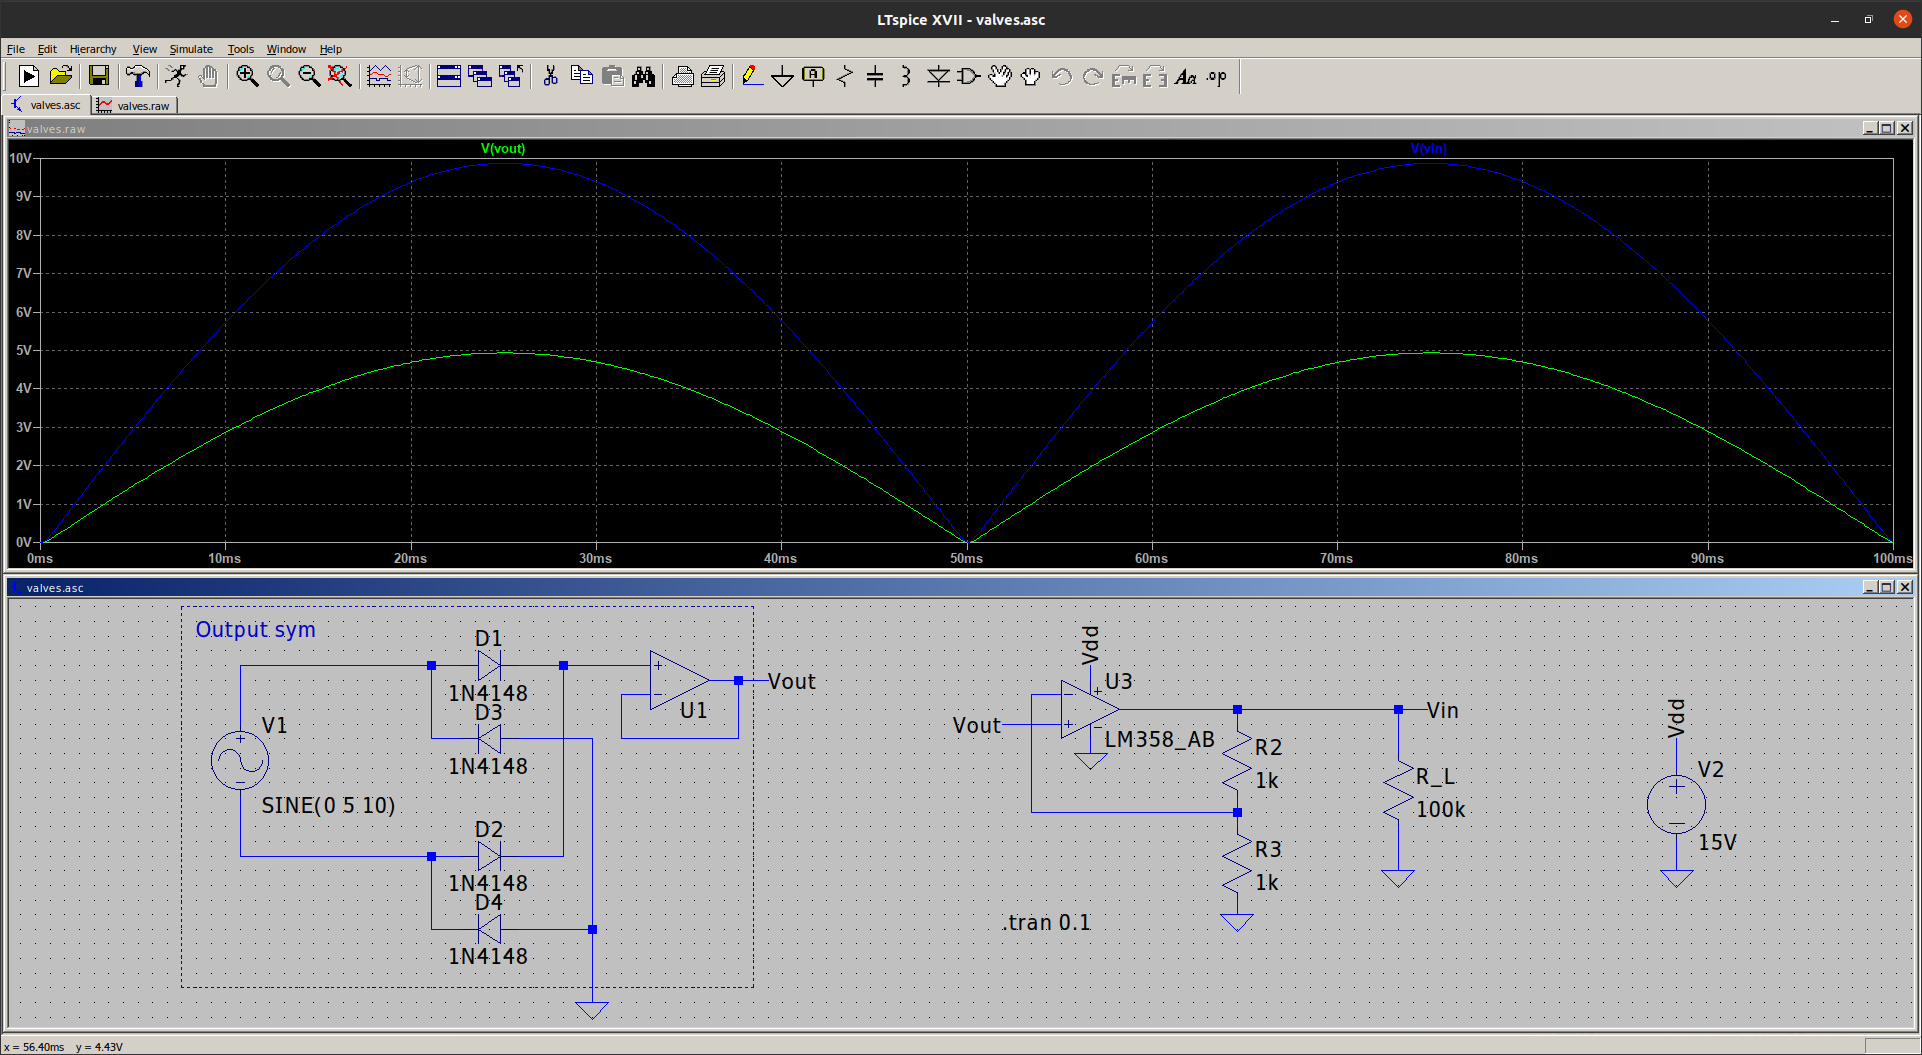
\includegraphics[width=0.8\textwidth]{imagens/valves_circ.png}
    \caption{Circuito de acionamento dos conjuntos das válvulas e resultados da simulação. A saída \emph{Vout} foi tal que simule uma varredura da saída analógica da placa de acionamento. O nó \emph{Vin} simula a entrada do atuador junto da impedância interna \emph{R\_L}.}
    \label{fig:imagens-valves_circ-png}
\end{figure}

\paragraph{Simulação}\mbox{}

Supôs-se que a limitação de velocidade da válvula é relativa à velocidade rotacional do motor, ou seja, o motor opera a 1º\,/\,s. Dessa forma, o tempo de resposta foi simulado com pequenos incrementos do valor do ângulo de abertura da válvula até que se atingisse o valor desejado. Além, é claro, da simulação do condicionamento do sinal.

